\documentclass{article}
\usepackage{cmap}
\usepackage[utf8]{inputenc}
\usepackage[english,ukrainian]{babel}
\usepackage{graphicx}
\usepackage{geometry}
\usepackage{listings}
\usepackage{float}
\usepackage{amsmath}
\geometry{
	a4paper,
	left=20mm,
	right=20mm,
	top=15mm,
	bottom=15mm,
}
\lstset{
	language=c,
	tabsize=4,
	keepspaces,
	showstringspaces=false,
}
\graphicspath{ {./pictures} }
\setlength{\parindent}{4em}

\newcommand\subject{Організація комп’ютерних мереж}
\newcommand\lecturer{асистент кафедри ПЗ \\ Задорожний І.М.}
\newcommand\teacher{асистент кафедри ПЗ \\ Задорожний І.М.}
\newcommand\mygroup{ПЗ-22}
\newcommand\lab{1}
\newcommand\theme{Налаштування протоколу ІР в Windows XP, дослідження роботи протоколу
	ARP}
\newcommand\purpose{Ознайомитися із засобами перевірки та налаштування протоколів TCP/IP та
	ARP}

\begin{document}
\begin{normalsize}
	\begin{titlepage}
		\thispagestyle{empty}
		\begin{center}
			\textbf{МІНІСТЕРСТВО ОСВІТИ І НАУКИ УКРАЇНИ\\
				НАЦІОНАЛЬНИЙ УНІВЕРСИТЕТ "ЛЬВІВСЬКА ПОЛІТЕХНІКА"}
		\end{center}
		\begin{flushright}
			\textbf{ІКНІ}\\
			Кафедра \textbf{ПЗ}
		\end{flushright}
		\vspace{200pt}
		\begin{center}
			\textbf{ЗВІТ}\\
			\vspace{10pt}
			до лабораторної роботи № \lab\\
			\textbf{на тему}: “\textit{\theme}”\\
			\textbf{з дисципліни}: “\subject”
		\end{center}
		\vspace{112pt}
		\begin{flushright}
			
			\textbf{Лектор}:\\
			\lecturer\\
			\vspace{28pt}
			\textbf{Виконав}:\\
			
			студент групи \mygroup\\
			Коваленко Д.М.\\
			\vspace{28pt}
			\textbf{Прийняв}:\\
			
			\teacher\\
			
			\vspace{28pt}
			«\rule{1cm}{0.15mm}» \rule{1.5cm}{0.15mm} 2023 р.\\
			$\sum$ = \rule{1cm}{0.15mm}……………\\
			
		\end{flushright}
		\vspace{\fill}
		\begin{center}
			\textbf{Львів — 2023}
		\end{center}
	\end{titlepage}
		
	\begin{description}
		\item[Тема.] \theme.
		\item[Мета.] \purpose.
	\end{description}

\section*{Теоретичні відомості}
\begin{enumerate}
	\item Як користуватися діалоговим вікном для задавання фільтрів?
	
	У полі Filter необхідно ввести потрібні фільтри (назва протоколу, IP-адреса відправника чи отримувача тощо) і натиснути Enter. У випадку побудови складніштих фільтрів використувуються оперетори порівння (== (eq), != (ne), 
	> (gt), < (lt), >= (ge), <= (le)) та логічні оператори ( (and), || (or),  (xor), 
	! (not)).
	
	\item Який принцип роботи протоколу ARP?
	
	ARP-протокол дозволяє за відомою ІР-адресою визначити МАС-адресу. Спочатку протокол пробує знайти необхідну адресу у кеші ARP, якщо такої немає, то створюється широкомовний запит, тобто усім вузлам надсилається запитання яку фізичну адресу має вузол із даною ІР-адресою. Отримана адреса утримується протягом визначеного часу у кеші.
	
	\item Що буде в результаті виконання команди ipconfig/flushdns?
	
	Дана команда очищає кеш зіставлення імен DNS клієнта.
	
\end{enumerate}

	\section*{Хід виконання}
	\begin{enumerate}
\item	Відвідав сторінку whatismyip.com, за допомогою якої дізнався свою IP-адресу. З командного рядка виконав команду ipconfig (яка виводить IP-адресу). Зіставив IP-адреси, одержані зазначеними двома способами.
	
	\begin{figure}[H]
		\centering
		\includegraphics[scale=0.7]{1}
		\caption{ IP-адреса, використовуючи  whatismyip.com}
	\end{figure}

	\begin{figure}[H]
		\centering
		\includegraphics[scale=0.7]{2}
		\caption{IP-адреса, використовуючи  команду ipconfig}
	\end{figure}

\item	Відвідав сторінку speedtest.net. Відобразив фрагмент екранного знімка сторінки, де містяться дані про швидкість виконання процедури ping та передавання і прийому даних
	\begin{figure}[H]
		\centering
		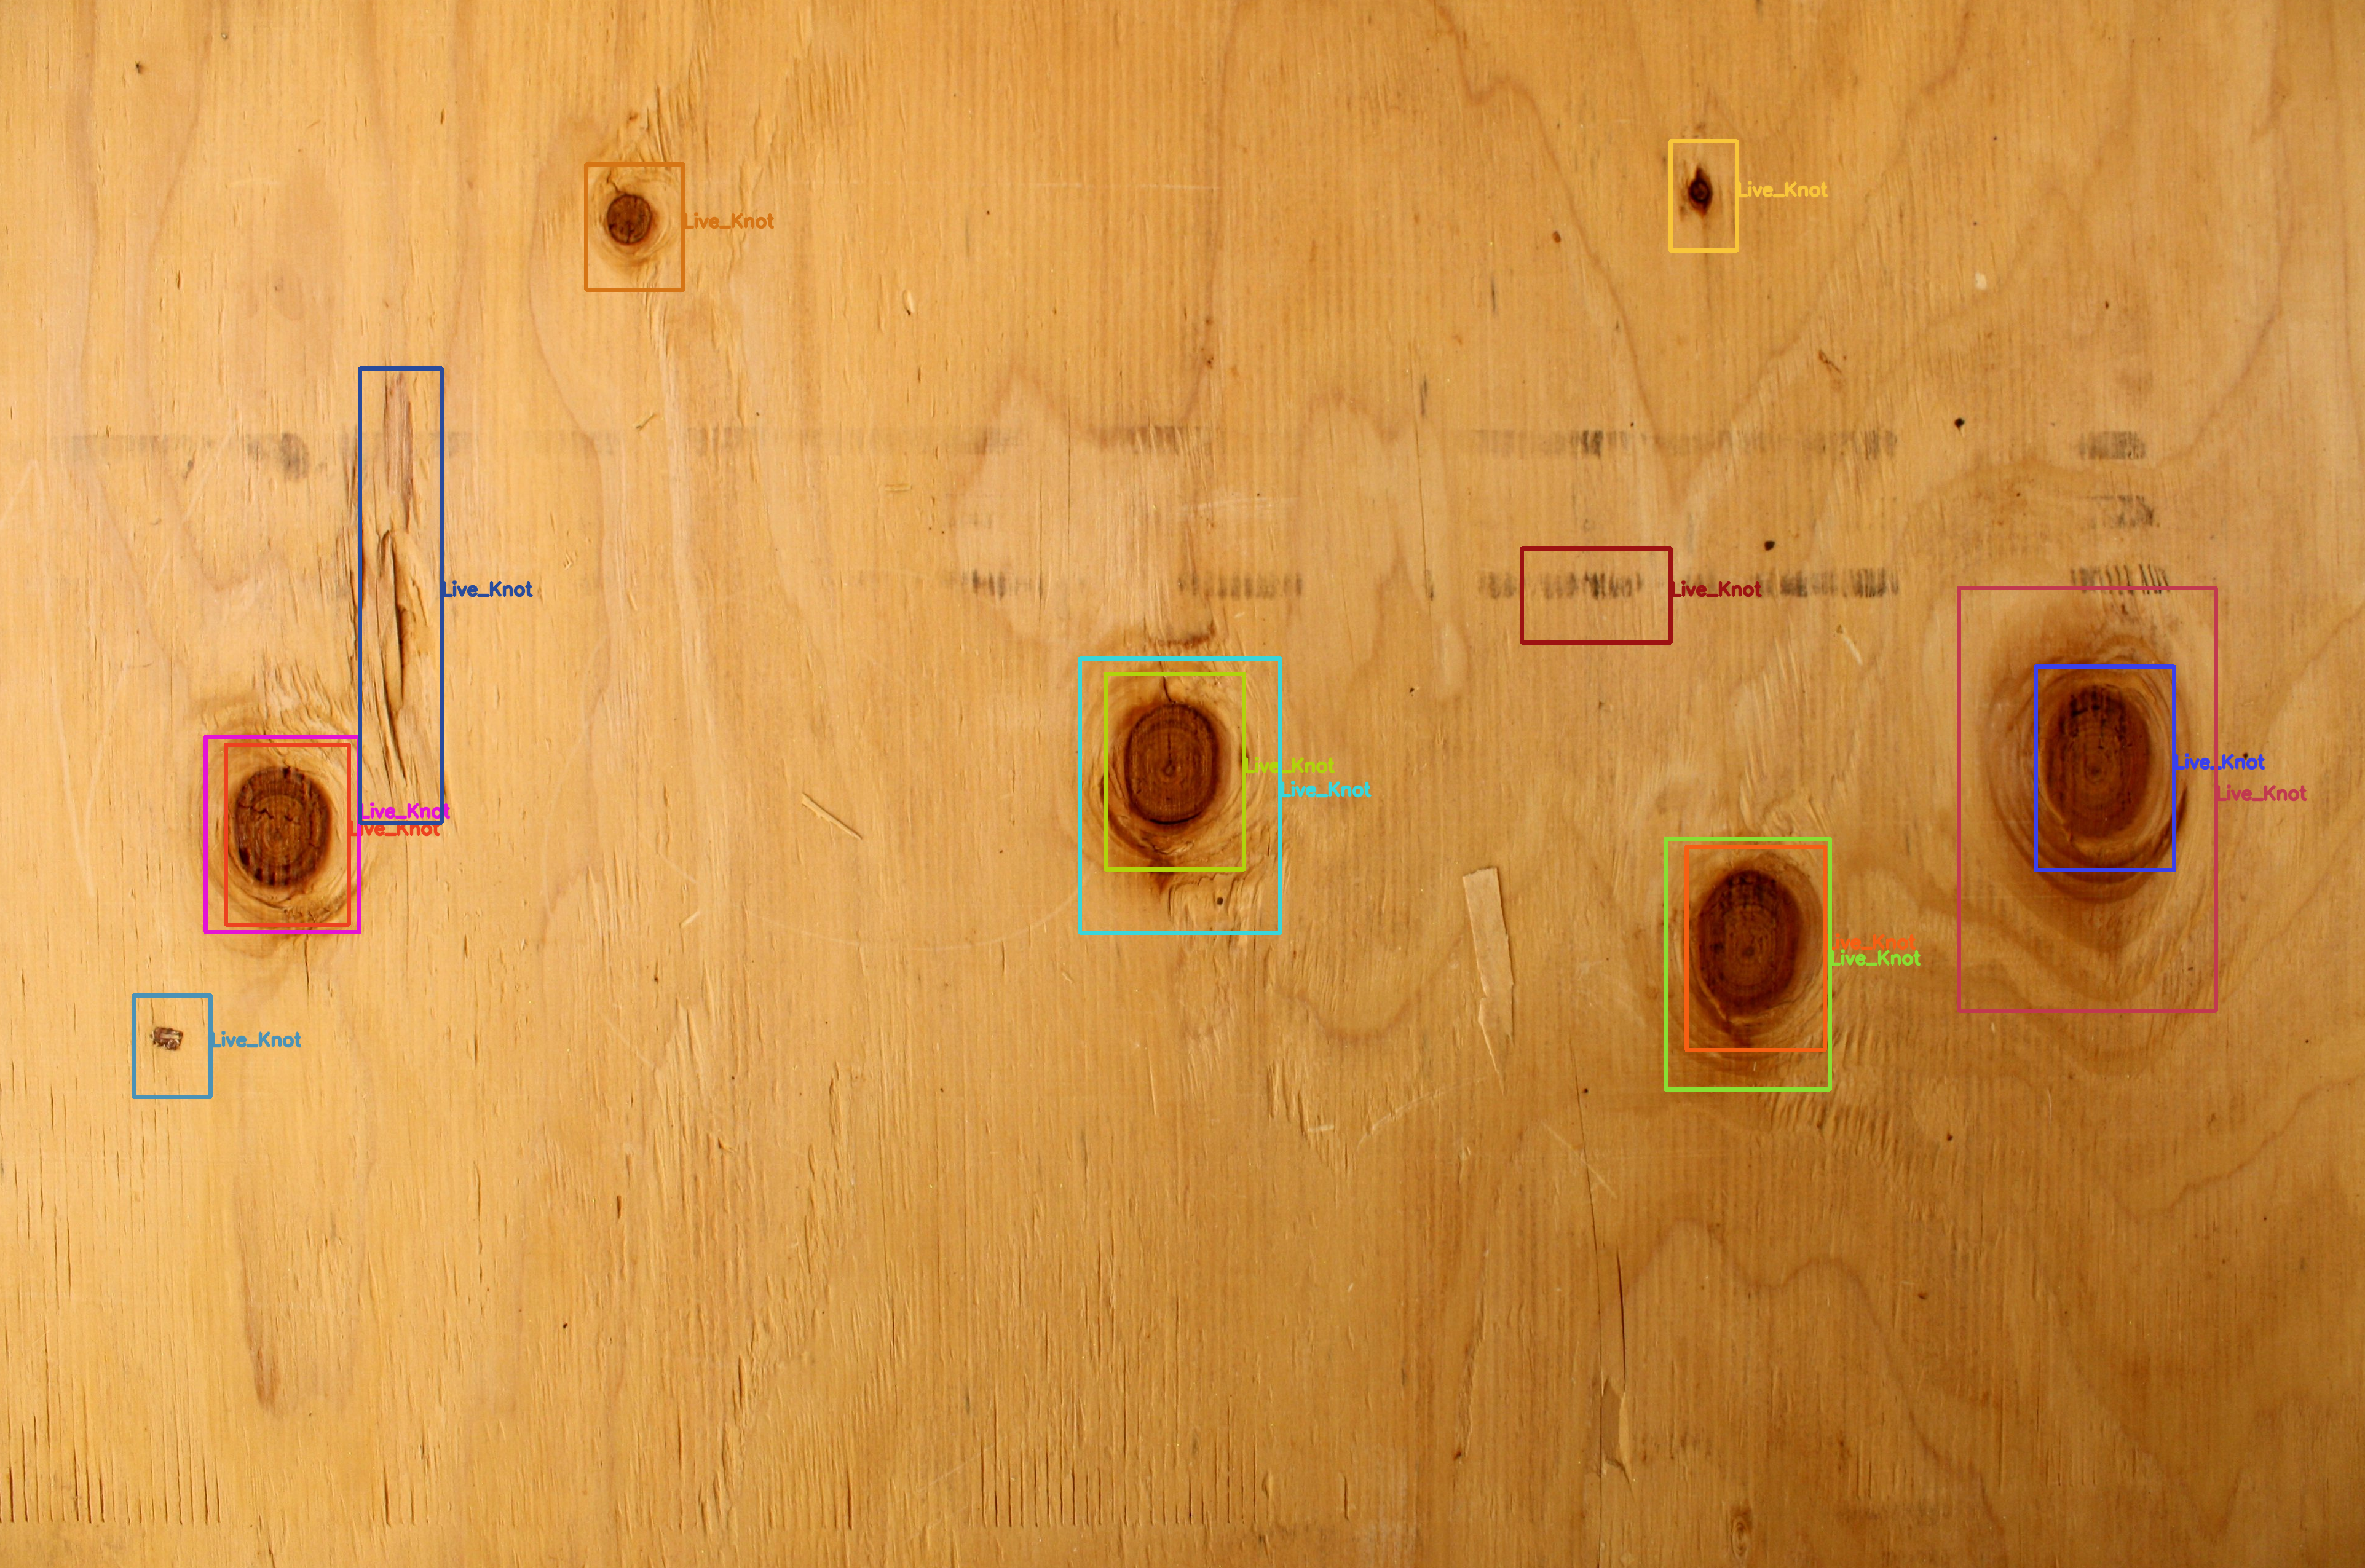
\includegraphics[scale=0.6]{3}
		\caption{Результати виконання Speedtest.net}
	\end{figure}
	
	\begin{figure}[H]
		\centering
		\includegraphics[scale=0.6]{13}
		\caption{Результати виконання процедури ping}
	\end{figure}

\item З командного рядка виконав команду ipconfig з параметром /all. 
	\begin{figure}[H]
	\centering
	\includegraphics[scale=0.6]{4}
	\caption{Результати виконання ipconfig з параметром /all
	}
\end{figure}

\item З командного рядка виконав спочатку команду ipconfig з параметром /displaydns, а тоді – з параметром /flushdns. 
	\begin{figure}[H]
	\centering
	\includegraphics[scale=0.7]{5}
	\caption{Результати виконання ipconfig з параметром /displaydns
	}
\end{figure}
\begin{figure}[H]
	\centering
	\includegraphics[scale=0.7]{6}
	\caption{Результати виконання ipconfig з параметром /flushdns
	}
\end{figure}

\item Виконав команду ipconfig з параметрами /renew та /release
\begin{figure}[H]
	\centering
	\includegraphics[scale=0.7]{7}
	\caption{Результати виконання ipconfig з параметром /renew
	}
\end{figure}
\begin{figure}[H]
	\centering
	\includegraphics[scale=0.7]{8}
	\caption{Результати виконання ipconfig з параметром /release
	}
\end{figure}
\item З командного рядка виконав команду arp.
\begin{figure}[H]
	\centering
	\includegraphics[scale=0.7]{9}
	\caption{Результати виконання arp
	}
\end{figure}
\item Налаштував необхідний мінімум параметрів, запустив процес перехоплення мережевого трафіка. Поспостерігав за процесом протягом декількох хвилин. Відфільтрував пакети, передані за протоколом ARP.
\begin{figure}[H]
	\centering
	\includegraphics[scale=0.6]{10}
	\caption{Результати фільтрування пакетів за протоколом ARP}
\end{figure}

\item Відмінив попередній фільтр. Знаючи свою IP-адресу, відфільтрував дані лише про пакети, передані з цієї адреси або ж прийняті на цю адресу
\begin{figure}[H]
	\centering
	\includegraphics[scale=0.5]{11}
	\caption{Результати фільтрування пакетів за IP-адресою}
\end{figure}
\item Знайти HTTP-запит і детально розглянути його
\begin{figure}[H]
	\centering
	\includegraphics[scale=0.5]{12}
	\caption{Результати фільтрування http пакетів}
\end{figure}
	\end{enumerate}

\section*{Висновки}
Під час виконання лобораторної роботи я провів ознайомлення із засобами перевірки та налаштування протоколів TCP/IP та ARP.
Отримав ІР-адреси на сайті whatismyip.com та за допопогою команди ipconfig, що відрізняються, оскільки у першому випадку отримано зовнішню ІР-адресу, а в іншому – локальну.
При виконанні команди ipconfig/flushdns я очистили кеш зіставлення імен DNS клієнта і тому при повторному виконанні ipconfig/displaydns я отримуємо порожній список.
ipconfig/release повідомляє, що клієнт більше не потребує своєї мережевої адреси, а ipconfig/renew надає нову адресу.
	    
\end{normalsize}
\end{document}
